\begin{figure}[h] \centering
	\centering
	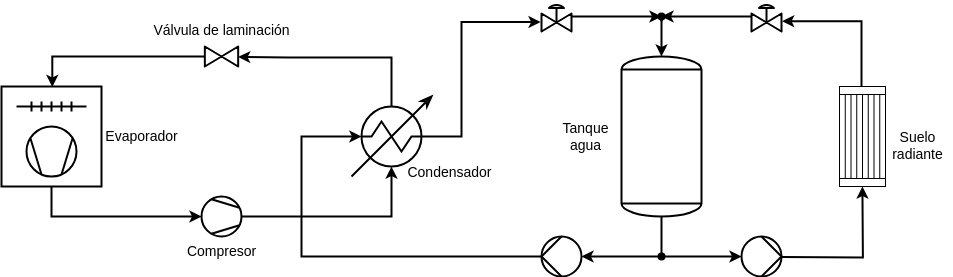
\includegraphics[width=1\textwidth]{./capitulos/resultados_discusion/images/sistema_termico.png}
	\caption{Esquema térmico.}
	\label{fig:thermal_diagram}
\end{figure}

Una bomba de calor produce agua caliente sanitaria que se vuelca en un depósito acumulador.
De este se extraen dos flujos, uno de vuelta al intercambiador de calor del condensador
de la bomba de calor ($\dot{m}_{cond}$), y otro que se dirige al suelo radiante ($\dot{m}_{cale}$).

Estos dos caudales se controlan a través de dos bombas de circulación y
posiblemente también con el uso de válvulas de estrangulación, si las bombas no
fueran de velocidad variable (VFD, Variable Frequency Drive).

La temperatura del tanque de agua es $T_{tanque}$, a la salida de la calefacción
del suelo radiante $T_{cale}$, y a continuación del condensador $T_{cond}$.

\subsection{Bomba de calor}

En lugar de modelar detalladamente la bomba de calor con sus componentes
(evaporador, compresor, condensador y válvula de expansión), se ha optado por
aproximar el COP (Coeficiente de Rendimiento) utilizando datos de hojas
técnicas. El COP se expresa en función de la temperatura de salida del agua del
condensador, denominada $T_{cond}$.

Según los datos de una bomba de calor comercial
\footnote{\url{https://www.daikin.es/content/dam/DACS/document-library/Pdfs-subidos-2022/Monobloc\%20EBLA\%209-11\%20-\%2014-16.pdf}}
el COP es 4.8 para una temperatura de 35°C y 3.4 para 55°C.
Se ha asumido una variación lineal del COP entre estos puntos, con un valor
mínimo de 0 y un máximo de 4.8.

La función por tramos que describe el COP es:

\begin{equation}
	\text{\text{cop}}(T) =
	\begin{cases}
		4.8              & \text{si } T < 35^\circ C                    \\[10pt]
		26.36 + -0.069 T & \text{si } 35^\circ C \leq T < 103.5^\circ C \\[10pt]
		0                & \text{si } T \geq 103.5^\circ C
	\end{cases}
\end{equation}

que se muestra en la figura \ref{fig:heat_pump_cop}

\begin{figure}[h] \centering
	\centering
	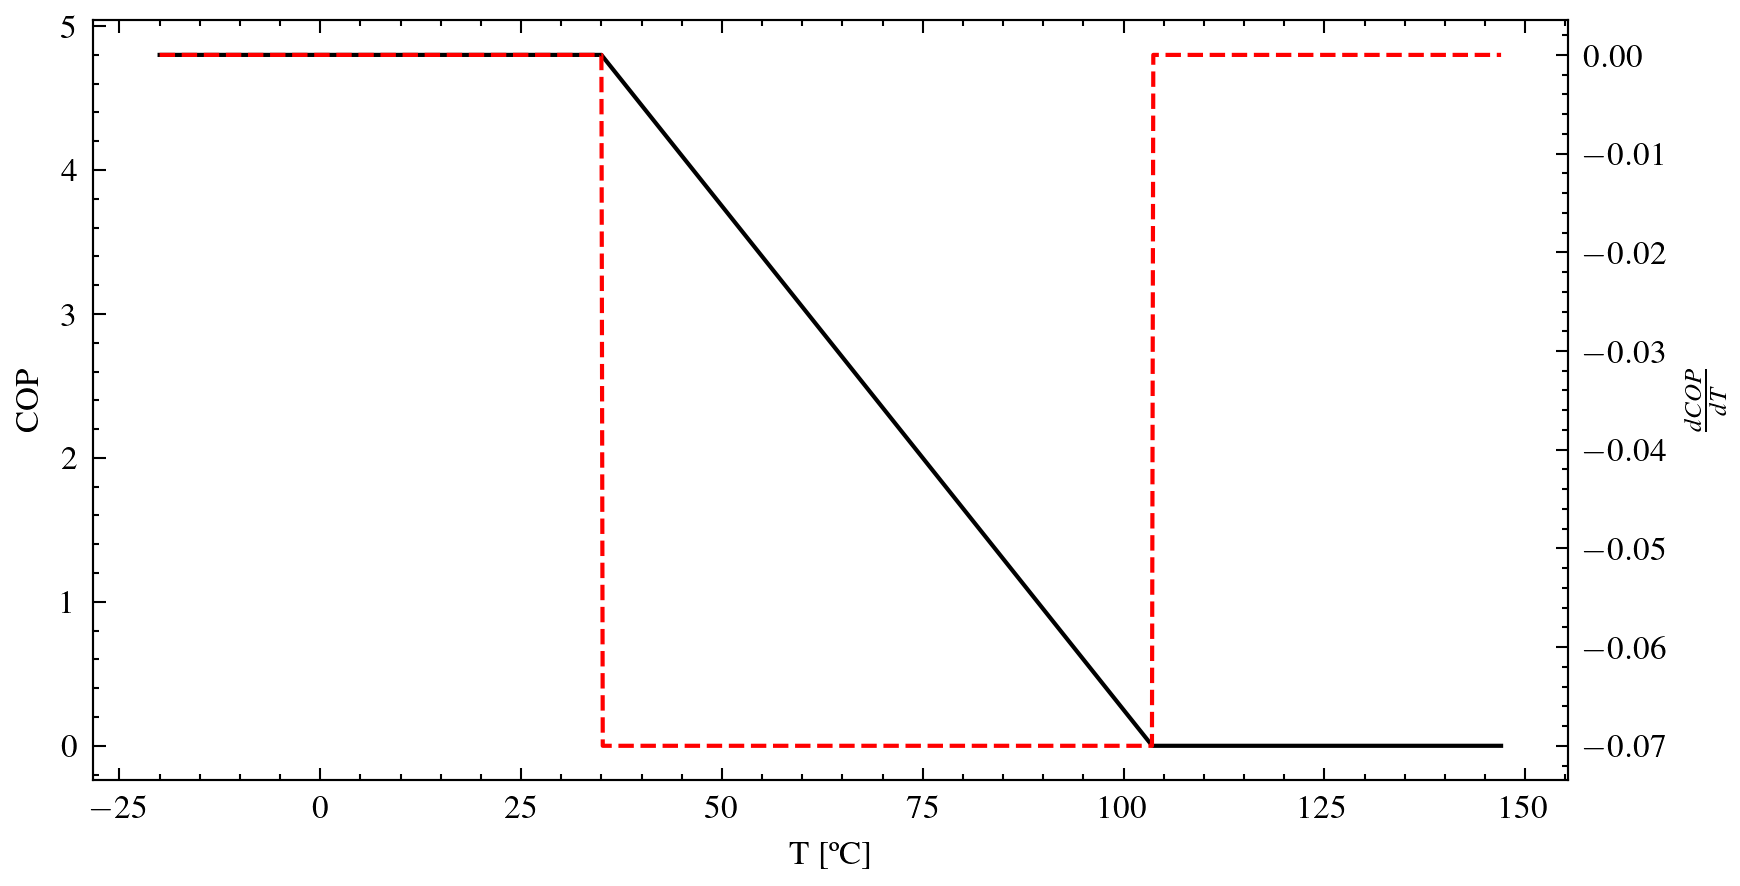
\includegraphics[width=1\textwidth]{./capitulos/resultados_discusion/images/heat_pump_cop.png}
	\caption{COP de la bomba de calor según la temperatura de salida del agua.
		Eje de ordenadas derecho muestra la derivada del COP respecto de la
		temperatura.}
	\label{fig:heat_pump_cop}
\end{figure}


\subsection{Tanque de agua}

Desde el depósito de agua aislado, tenemos dos flujos de entrada y salida
controlados por dos bombas de circulación. Un caudal para la bomba de calor
$\dot{m}_{cond}$, y otro para el suelo radiante $\dot{m}_{suelo}$.

La ecuación de conservación de la energía para el tanque con pérdidas de calor
por conducción con el ambiente (suponemos que se encuentra en el exterior de la
vivienda) es

\begin{align} \label{eq:t_tanque_balance}
	m_{tanque} \cdot cp_{agua} \cdot \left( \frac{dT_{tanque}}{dt} \right) & = \dot{m}_{cond} \cdot cp_{agua} \cdot T_{cond} \nonumber     \\
	                                                                       & + \dot{m}_{cale} \cdot cp_{agua} \cdot T_{cale} \nonumber     \\
	                                                                       & - \dot{m}_{tanque} \cdot cp_{agua} \cdot T_{tanque} \nonumber \\
	                                                                       & - \dot{Q}_{perdida}
\end{align}

con las ecuaciones

\begin{align}
	\text{COP}        & = \text{cop}(T_{cond})         \label{eq:cop_t_cond}                               \\
	\dot{Q}_{cond}    & = \text{COP} \cdot P_{bomba}   \label{eq:q_cond_1}                                 \\
	\dot{Q}_{cond}    & = \dot{m}_{cond} \cdot cp_{agua} \cdot (T_{cond} - T_{tanque}) \label{eq:q_cond_2} \\
	\dot{m}_{tanque}  & = \dot{m}_{cond} + \dot{m}_{cale}      \label{eq:m_dot_tanque}                     \\
	\dot{Q}_{perdida} & = U_{tanque} \cdot A_{tanque} \cdot (T_{tanque} - T_{amb})  \label{eq:q_perdida}
\end{align}

donde

\begin{itemize}
	\item $\text{COP}$: Coeficiente de rendimiento.
	\item $\text{cop}(T_{cond})$: Función que define el COP en función de $T_{cond}$.
	\item $m_{tanque}$: Masa del tanque.
	\item $cp_{agua}$: Calor específico del agua.
	\item $\dot{m}_{tanque}$: Flujo másico del tanque.
	\item $\dot{m}_{cond}$: Flujo másico del condensador.
	\item $\dot{m}_{cale}$: Flujo másico de suelo radiante, calefacción.
	\item $T_{tanque}$: Temperatura del tanque.
	\item $T_{cond}$: Temperatura a la salida el condensador.
	\item $T_{cale}$: Temperatura calefacción, a la salida del suelo radiante.
	\item $T_{amb}$: Temperatura ambiente.
	\item $\dot{Q}_{perdida}$: Pérdidas de calor del depósito por conducción.
	\item $\dot{Q}_{cond}$: Tasa de transferencia de calor en el condensador.
	\item $P_{bomba}$: Potencia del compresor.
	\item $U_{tanque}$: Coeficiente global de transferencia de calor del tanque.
	\item $A_{tanque}$: Área de la superficie del tanque.
\end{itemize}


\subsection{Suelo radiante}

Del depósito de agua hacemos circular un caudal de agua caliente por los
tubos del suelo radiante, que se encuentran incrustados en una losa de hormigón
sobre una superficie aislante.

Esta losa de hormigón que da una inercia térmica considerable al suelo, se ha
tomado de 5cm. Y tampoco hemos considerado que se haya recubierto la losa de
hormigón con ningún azulejo, porcelánico o madera.

\begin{figure}[h] \centering
	\centering
	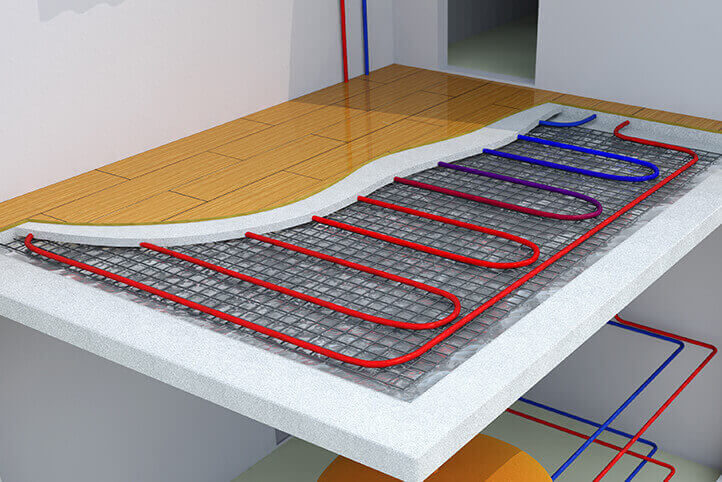
\includegraphics[width=1\textwidth]{./capitulos/resultados_discusion/images/radiant_heating_floor.jpg}
	\caption{Suelo radiante. Fuente: \url{https://www.palodurohardwoods.com/blog/radiant-heat/}}
	\label{fig:radiant_heating_floor}
\end{figure}

El suelo calienta la habitación (el aire de la habitación) principalmente por
radiación y en menor medida por convección natural, despreciándose la
transferencia de calor por conducción.

De forma que el aire de la casa también tiene una inercia térmica, y pierde
calor por las paredes, tejado y ventanas.

Las ecuaciones del balance térmico del suelo y habitación por tanto también
están acopladas y son:

\begin{align} \label{eq:floor_energy_conservation}
	m_{suelo} \cdot cp_{suelo} \cdot \left( \frac{dT_{suelo}}{dt} \right) & = \dot{Q}_{conduccion-suelo} \nonumber \\
	                                                                      & - \dot{Q}_{conveccion-suelo} \nonumber \\
	                                                                      & - \dot{Q}_{radiacion-suelo}
\end{align}

\begin{align} \label{eq:room_energy_conservation}
	m_{aire} \cdot cp_{aire} \cdot \left( \frac{dT_{habitacion}}{dt} \right) & = \dot{Q}_{conveccion-suelo} \nonumber                                       \\
	                                                                         & + \dot{Q}_{radiacion-suelo} \nonumber                                        \\
	                                                                         & - U_{paredes} \cdot A_{paredes} \cdot (T_{habitacion} - T_{amb}) \nonumber   \\
	                                                                         & - U_{techo} \cdot A_{techo} \cdot (T_{habitacion} - T_{amb}) \nonumber       \\
	                                                                         & - U_{ventanas} \cdot A_{ventanas} \cdot (T_{habitacion} - T_{amb})
\end{align}

donde la transferencia de calor por conducción desde el agua caliente que
circula por los tubos hasta el suelo de hormigón viene dada por:

\begin{align} \label{eq:q_conduccion_1}
	\dot{Q}_{conduccion-suelo} & = \dot{m}_{cale} \cdot cp_{agua} \cdot (T_{tanque} - T_{cale})
\end{align}
\begin{align} \label{eq:q_conduccion_2}
	\dot{Q}_{conduccion-suelo} & = U_{tubos} \cdot A_{tubos} \cdot \Delta T_{tubos}
\end{align}

la diferencia de temperaturas representativa $\Delta T_{tubos}$ para un
intercambiador de calor sin cambios de fase se suele tomar como el LMTD (Log
Mean Temperature Difference):

\begin{equation} \label{eq:lmtd}
	\Delta T_{tubos} = \frac{(T_{tanque} - T_{suelo-salida}) - (T_{cale} - T_{suelo-entrada})}{\ln\left(\frac{T_{tanque} - T_{suelo-salida}}{T_{cale} - t_{suelo-entrada} } \right) }
\end{equation}

pero en nuestro caso hemos tomado que la temperatura del suelo se mantiene
constante a lo largo del recorrido de los tubos (figura
\ref{fig:floor_temperatures}), lo que nos aproxima más al caso de un
intercambiador de calor con cambio de fase, y por tanto hemos tomado la
diferencia de temperaturas media como la representativa

\begin{equation} \label{eq:mean_delta_T}
	\Delta T_{tubos} = \frac{(T_{tanque} - T_{suelo}) + (T_{cale} - T_{suelo})}{2}
\end{equation}

\begin{figure}[h] \centering
	\centering
	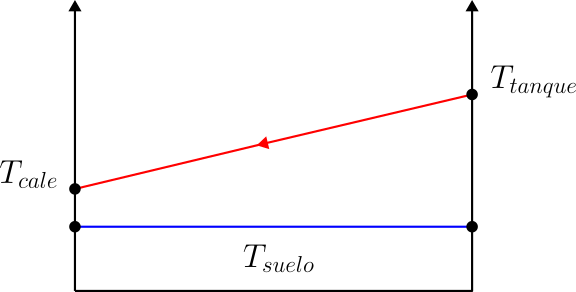
\includegraphics[width=0.6\textwidth]{./capitulos/resultados_discusion/images/floor_temperatures.png}
	\caption{Evolución de temperaturas para el suelo radiante.}
	\label{fig:floor_temperatures}
\end{figure}

y $U_{tubos}$ es la transmitancia térmica, que se considera constante para todo
el tramo del interambiador de calor, y es igual a:

\begin{equation}
	U_{tubos} = \frac{1}{\left( \frac{1}{\frac{k_{pex}}{t_{tubo}}} \right) + \left( \frac{1}{h_{tubo}} \right)}
\end{equation}

donde

\begin{itemize}
	\item $k_{pex}$: coeficiente de conductividad térmica del polietileno reticulado (PEX), igual a $0.41\left[ \frac{W}{m \cdot K} \right]$.
	\item $t_{tubo}$: Grosor del tubo de $0.635[cm]$ para tubo PEX de una pulgada.
	\item $h_{tubo}$: Coeficiente de pelicula para la transferencia de calor por convección entre el agua y los tubos.
\end{itemize}

y a su vez el coeficiente de película $h_{tubo}$ lo averiguamos del número de
Nusselt, y la ecuación de Dittus-Boelter \eqref{eq:dittus-boelter} que
relaciona los números de Prandtl, Reynolds y el Nusselt en flujo turbulento
para tubos circulares (encontrada en Incropera et al.
\cite{incropera1996fundamentals}). De forma que también asumimos que estaremos
siempre en régimen turbulento.

\begin{align}
	\text{Nu}_{tubo} & = \frac{h_{tubo} \cdot D_{tubo}}{k_{agua}}                                                                                   \\
	\text{Nu}_{tubo} & = 0.023 \cdot \text{Re}_{tubo}^{0.8} \cdot \text{Pr}_{agua}^{0.3}     \label{eq:dittus-boelter}                              \\
	\text{Re}_{tubo} & = \frac{D_{tubo} \cdot v \cdot \rho_{agua}}{\mu_{agua}} = \frac{4 \cdot \dot{m}_{cale}}{\pi \cdot \mu_{agua} \cdot D_{tubo}}
\end{align}

teniendo

\begin{itemize}
	\item $D_{tubo}$: diámetro interior del tubo de PEX.
	\item $k_{agua}$: conductividad térmica del agua a 300 Kelvin, igual a $0.6\left[\frac{W}{m \cdot K}\right]$.
	\item $\text{Pr}_{agua}$: Prandtl para el agua a 300 Kelvin. Valor de 6.9 adimensional.
	\item $v$: Velocidad del agua por los tubos.
	\item $\rho_{agua}$: densidad del agua a $300[K]$, de aproximadamente $1000\left[\frac{kg}{m^3}\right]$.
	\item $\mu_{agua}$: viscosidad dinámica del agua a $320[K]$, valiendo $0.000577[Pa \cdot s]$.
\end{itemize}


Y las transferencias de calor por radiación y convección natural de las
ecuaciones \eqref{eq:floor_energy_conservation} y
\eqref{eq:room_energy_conservation}, son:

\begin{align} \label{eq:q_radiacion}
	\dot{Q}_{radiacion-suelo} & =  \sigma \cdot \epsilon_{hormigon} \cdot A_{suelo} \cdot (T_{suelo}^4 - T_{habitacion}^4)
\end{align}

\begin{align} \label{eq:q_conveccion}
	\dot{Q}_{conveccion-suelo} & = h_{suelo} \cdot A_{suelo} \cdot (T_{suelo} - T_{habitacion})
\end{align}

con los coeficientes:

\begin{itemize}
	\item $\sigma$: constante de Stefan-Boltzmann: $5.67\cdot 10^{-8} \left[\frac{W}{m^2 \cdot K^4}\right]$.
	\item $\epsilon_{hormigon}$: emisividad del hormigón a 300 Kelvin de 0.93 (adimensional).
	\item $A_{suelo}$: superficie del suelo, $100[m^2]$.
\end{itemize}

y el coeficiente de película $h_{suelo}$ de transferencia de calor por
convección natural entre el suelo y aire de la habitación lo obtenemos
igualmente por el Nusselt, y la relación empírica
\eqref{eq:empirical_nu_natural_convection} para placas horizontales (dada en
Cengel et al. \cite{cengel2007transferencia}):

\begin{align}
	\text{Nu}_{suelo} & = \frac{h_{suelo} \cdot L}{k_{aire}}                                                    \\
	\text{Nu}_{suelo} & = 0.15 \cdot \text{Ra}_{aire}^{\frac{1}{3}}  \label{eq:empirical_nu_natural_convection} \\
	\text{Ra}_{aire}  & = \text{Gr}_{aire} \cdot \text{Pr}_{aire}                                               \\
	\text{Gr}_{aire}  & = \frac{g \cdot \beta \cdot ( T_{suelo} - T_{habitacion} ) \cdot L^3}{\nu_{aire}^2}
\end{align}


donde

\begin{itemize}
	\item $\text{Nu}$: número de Nusselt.
	\item $\text{Gr}$: número de Rayleigh.
	\item $\text{Gr}$: número de Grashof.
	\item $L$: longitud característica, relación entre el área del suelo y su
	      perímetro, igual al ancho del área del suelo para planta cuadrada
	      ($10[m]$).
	\item $k_{aire}$: conductividad térmica del aire a 300 Kelvin, $0.0263\left[ \frac{W}{m \cdot K} \right]$.
	\item $g$: aceleración de la gravedad, $9.8\left[\frac{m}{s^2}\right]$
	\item $\beta$: coeficiente de expansión volumétrica para el aire, que
	      tratamos como un gas ideal a $300[K]$, y por tanto calculamos como $\beta =
		      \frac{1}{T} = \frac{1}{300} \left[K^{-1}\right]$.
	\item $\nu_{aire}$: viscosidad cinemática del aire a 300 Kelvin: $15.89 \cdot 10^{-6} \left[\frac{m^2}{s}\right]$.
\end{itemize}
